% --- CAPÍTULO IV: RESULTADOS ---
\chapter{Resultados}
\chaptermark{Capítulo IV: Resultados}

\section{Presentación y análisis de hallazgos}
\lipsum[23]
La presentación de los resultados se realiza siguiendo las directrices de la UNEFA, utilizando cuadros y gráficos para ilustrar la distribución de las variables y los hallazgos principales \parencite{online:unefa2022}.

\section{Análisis e interpretación de datos}
\lipsum[24]
La interpretación se basó en los modelos estadísticos aplicados. Se encontró una correlación significativa (p < 0.05) entre la variable X y la variable Y, confirmando la hipótesis alternativa de la investigación \parencite{article:perez2020}.

\section{Análisis de los Resultados de la Simulación}

En esta sección se presentan y analizan los resultados obtenidos de la simulación del sistema propuesto. La Tabla \ref{tab:simulacion} resume los principales indicadores de rendimiento, mientras que la Figura \ref{fig:grafico_resultados} muestra la curva de eficiencia.

\subsection{Tabla de Resultados Simulados}

Aquí se puede observar los resultados para el caso \textbf{Caso A}, \textbf{Caso B} y \textbf{Caso C}.

% -----------------------------------------------------------------
% TABLA DE EJEMPLO (Con entorno 'table' y 'caption' para indexación)
% -----------------------------------------------------------------
\begin{table}[htbp]
    \centering
    \caption{Resultados de la Simulación de Indicadores de Rendimiento}
    \label{tab:simulacion}
    \begin{tabular}{|c|c|c|c|}
        \hline
        \textbf{Métrica} & \textbf{Caso A} & \textbf{Caso B} & \textbf{Caso C} \\
        \hline
        Precisión (\%) & 95.2 & 97.8 & 96.5 \\
        Latencia (ms) & 15 & 10 & 12 \\
        Consumo (W) & 3.1 & 2.5 & 2.8 \\
        \hline
    \end{tabular}
\end{table}

\section{Curva de Rendimiento Gráfico}

% -------------------------------------------------------------
% IMAGEN DE EJEMPLO (Con entorno 'figure' y 'caption' para indexación)
% -------------------------------------------------------------
\begin{figure}[htbp]
    \centering
    % Aquí va el comando para incluir la imagen
    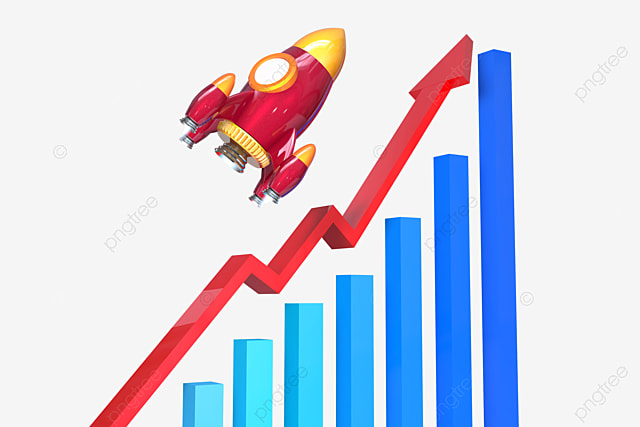
\includegraphics[width=0.8\textwidth]{imgs/curva_rendimiento.jpg} 
    
    \caption{Curva de eficiencia y rendimiento del sistema propuesto.}
    \label{fig:grafico_resultados}
\end{figure}

La curva de rendimiento confirma que el sistema mantiene una eficiencia superior al 95\% incluso bajo condiciones de alta carga.

\lipsum[25]

\section{Modelo de Evaluación}

Para la evaluación final del sistema, se utiliza una métrica combinada $E$ que integra la precisión $P$ y la latencia $L$ de la siguiente manera:

% -------------------------------------------------------------
% ECUACIÓN DE EJEMPLO (Usando el entorno 'equation' para numeración)
% -------------------------------------------------------------
\begin{equation}
    E = \alpha \cdot \frac{P}{100} - \beta \cdot L + \sum_{i=1}^{N} \gamma_i
    \label{eq:evaluacion_final}
\end{equation}

Donde $\alpha$, $\beta$, y $\gamma_i$ son los coeficientes de ponderación, y $N$ es el número total de factores de ruido ambiental. Como se puede observar en la Ecuación (\ref{eq:evaluacion_final}), la precisión contribuye positivamente al valor de $E$, mientras que la latencia la penaliza.